\let\negmedspace\undefined
\let\negthickspace\undefined
\documentclass[journal]{IEEEtran}
\usepackage[a5paper, margin=10mm, onecolumn]{geometry}
%\usepackage{lmodern} % Ensure lmodern is loaded for pdflatex
\usepackage{tfrupee} % Include tfrupee package

\setlength{\headheight}{1cm} % Set the height of the header box
\setlength{\headsep}{0mm}     % Set the distance between the header box and the top of the text

\usepackage{gvv-book}
\usepackage{gvv}
\usepackage{cite}
\usepackage{amsmath,amssymb,amsfonts,amsthm}
\usepackage{algorithmic}
\usepackage{graphicx}
\usepackage{textcomp}
\usepackage{xcolor}
\usepackage{txfonts}
\usepackage{listings}
\usepackage{enumitem}
\usepackage{mathtools}
\usepackage{gensymb}
\usepackage{comment}
\usepackage[breaklinks=true]{hyperref}
\usepackage{tkz-euclide} 
\usepackage{listings}
% \usepackage{gvv}                                        
\def\inputGnumericTable{}                                 
\usepackage[latin1]{inputenc}                                
\usepackage{color}                                            
\usepackage{array}                                            
\usepackage{longtable}                                       
\usepackage{calc}                                             
\usepackage{multirow}                                         
\usepackage{hhline}                                           
\usepackage{ifthen}                                           
\usepackage{lscape}
\begin{document}

\bibliographystyle{IEEEtran}
\vspace{3cm}

\title{1-1.2-28}
\author{EE24BTECH11036 - Krishna Patil}
% \maketitle
% \newpage
% \bigskip
{\let\newpage\relax\maketitle}

\renewcommand{\thefigure}{\theenumi}
\renewcommand{\thetable}{\theenumi}
\setlength{\intextsep}{10pt} % Space between text and floats


\numberwithin{equation}{enumi}
\numberwithin{figure}{enumi}
\renewcommand{\thetable}{\theenumi}

\textbf { Question :- } \\
 In which quadrant or on which axis do each of the points {$ \brak{-2,4 }$}, {$ \brak{3,-1} $}, {$ \brak{-1,0} $}, {$ \brak{1,2} $} and {$ \brak{-3,-5} $} lie ? Verify your answer by locating them on the Cartesian plane. \\ \\
\textbf { Solution :- } \\
To determine if point lies in a quadrant , we look at the the signs of the x and y coordinates.
\begin{table}[h!]    
  \centering
  \begin{tabular}[12pt]{|c|c|c|}
    \hline
    Parameter & Description & Values\\ 
    \hline
    $V$ & $\myvec{ 1 & 0 \\ 0 & 1-e^{2} }$ & $\myvec{1 & 0 \\ 0 & \frac{4}{9} }$ \\
    \hline
    $u$ & - & $\myvec{0 \\ 0}$ \\
    \hline
    $f$ & $b^2(e^2 -1)$ & -4 \\
    \hline
    $A$ & Area under Curve & $6\pi$ \\
    \hline
    \end{tabular}

  \caption{Quadrant Decider}
  \label{tab1-1.2-28}
\end{table}
\begin{enumerate}
\item {$ \vec A $} = (-2,4) lies in second quadrant.
\item {$ \vec B $} = (3,-1)  lies in fourth quadrant.
\item {$ \vec C $} = (-1,0) lies on the x axis.
\item {$ \vec D $} = (1,2) lies in the first quadrant.
\item {$ \vec E $} = (-3,-5) lies in the third quadrant.
\end {enumerate} 
\begin{figure}[h!]
   \centering
   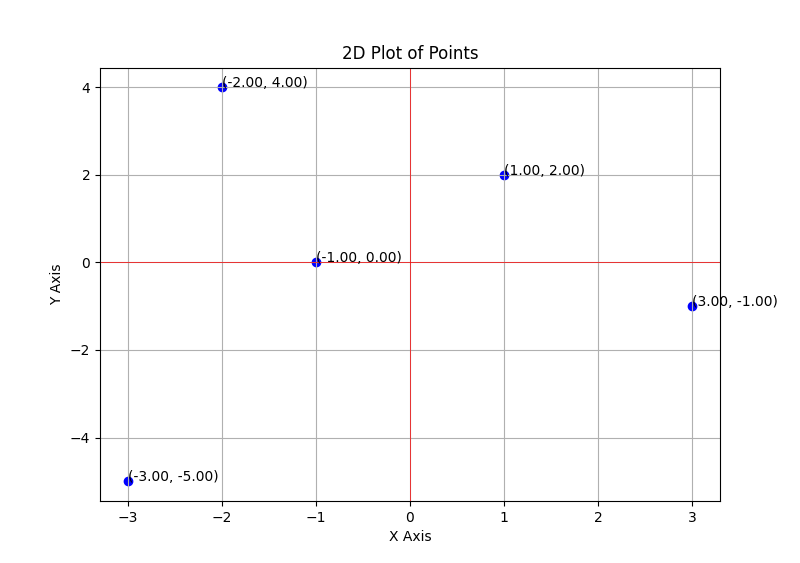
\includegraphics[width=0.6\linewidth]{figures/Figure_1.png}
   \label{x-yplot}
\end{figure}
\end{document}
